% !TEX root = task-1-13-4.tex
% Editable task bank. Append new BankTask blocks at the end of the document.
\documentclass[12pt,a4paper]{article}
\usepackage{physics-textbook}
\usepackage{graphicx,needspace}
\usetikzlibrary{decorations.pathmorphing}
\newif\ifShowSolutions
\ifdefined\TutorEdition
  \ShowSolutionstrue
\else
  \ShowSolutionsfalse % Change to \ShowSolutionstrue to display solutions.
\fi
\newcounter{banktask}
\newsavebox{\BankTaskBox}
\newcommand{\BankTaskContent}[3]{%
  \noindent\textbf{\thebanktask.}\quad #2\par
  \ifShowSolutions
    \Needspace{50mm}% Keep the solution heading with its opening text or diagram.
    #3\par
    \ifdefined\TutorEdition
      \ifcsname TutorSource#1\endcsname
        \nopagebreak\smallskip{\small\csname TutorSource#1\endcsname\par}%
      \fi
    \fi
  \fi
}
\newcommand{\BankTask}[3]{%
  \refstepcounter{banktask}\par\medskip
  \sbox{\BankTaskBox}{\begin{minipage}{\linewidth}%
    \BankTaskContent{#1}{#2}{#3}\end{minipage}}%
  \ifdim\dimexpr\ht\BankTaskBox+\dp\BankTaskBox\relax>\dimexpr\textheight-20mm\relax
    \Needspace{35mm}\BankTaskContent{#1}{#2}{#3}%
  \else
    \Needspace{\dimexpr\ht\BankTaskBox+\dp\BankTaskBox\relax}%
    \noindent\usebox{\BankTaskBox}\par
  \fi
  \medskip
}
\begin{document}
\BookSubsection{1.13.4}{Закон Архимеда}


% Source sdamgia-3559: https://phys-ege.sdamgia.ru/problem?id=3559
\BankTask{sdamgia-3559}{
Как изменится сила Архимеда при погружении тела на глубину, вдвое большую от исходного уровня? Жидкость считайте несжимаемой. Тело изначально полностью погружено в воду.\begin{enumerate}\item Увеличится в $2$ раза.\item Уменьшится в $2$ раза.\item Не изменится.\item Увеличится более чем в $2$ раза.\end{enumerate}
}{
\smallskip\noindent\textbf{Решение}\par
Согласно закону Архимеда, выталкивающая сила, действующая на погруженное в жидкость тело равна весу вытесненной жидкости: $F_A=\rho gV,$ здесь $\rho$ — плотность жидкости, а $V$ — объем тела. Поскольку жидкость можно считать несжимаемой, ее плотность с глубиной не изменяется, а значит, остается неизменной и сила Архимеда.
Ответ: $3$.
}

% Source sdamgia-19916: https://phys-ege.sdamgia.ru/problem?id=19916
\BankTask{sdamgia-19916}{
Деревянный кубик имеет ребро длиной $2\,\text{см}$. Определите архимедову силу, действующую на кубик при его полном погружении в воду.
}{
\smallskip\noindent\textbf{Решение}\par
Кубик имеет объем $V=a^3$. При полном погружении кубика архимедова сила равна:

$F_A=\rho_{\text{ж}}gV=\rho_{\text{ж}}ga^3=1000\cdot10\cdot0{,}02^3=0{,}08\,\text{Н}.$

Ответ: $0{,}08$.
}

% Source sdamgia-25020: https://phys-ege.sdamgia.ru/problem?id=25020
\BankTask{sdamgia-25020}{
На кусок алюминия массой $0{,}54\,\text{кг}$ при полном погружении в воду действует сила Архимеда, равная $2\,\text{Н}$. Чему равна при этом масса вытесненной воды?
}{
\smallskip\noindent\textbf{Решение}\par
Задание содержит избыточные данные, поэтому решить можно двумя способами.
$1$. По закону Архимеда выталкивающая сила равна весу вытесненной жидкости $F_A=m_{\text{ж}}g,$ откуда:

$m_{\text{ж}}=\frac{F_A}{g}=\frac2{10}=0{,}2\,\text{кг}.$

$2$. Объем вытесненной жидкости равен объему тела. Объем тела $V=\frac m{\rho_a}.$ Масса вытесненной жидкости:

$m_{\text{ж}}=\rho_{\text{в}}V=\frac{\rho_{\text{в}}m}{\rho_a}=\frac{1000\cdot0{,}54}{2700}=0{,}2\,\text{кг}.$

Ответ: $0{,}2$.
}

% Source sdamgia-24093: https://phys-ege.sdamgia.ru/problem?id=24093
\BankTask{sdamgia-24093}{
Наполненная газом сферическая резиновая оболочка полностью погружена в глубокий водоем и имеет радиус $75\,\text{см}$. Оболочку начинают погружать вглубь водоема, и через некоторое время ее радиус становится равным $25\,\text{см}$ (а форма остается сферической). Во сколько раз в результате такого погружения изменяется модуль действующей на оболочку силы Архимеда? Считайте изменение плотности воды с увеличением глубины пренебрежимо малым.
}{
\smallskip\noindent\textbf{Решение}\par
Сила Архимеда вычисляется по формуле $F_A=\rho gV.$ При этом оболочка имеет форму шара, объем которого равен:

$V=\frac43\pi R^3.$

Следовательно, сила Архимеда равна $F_A=\frac43\pi\rho gR^3.$ Из полученной формулы следует, что сила Архимеда пропорциональна кубу радиуса оболочки. Отсюда:

$\frac{F_{A1}}{F_{A2}}=\left(\frac{R_1}{R_2}\right)^3=\left(\frac{75}{25}\right)^3=27.$

 
Таким образом, сила Архимеда уменьшилась в $27$ раз.
 
Ответ: $27$.
}

% Source sdamgia-12930: https://phys-ege.sdamgia.ru/problem?id=12930
\BankTask{sdamgia-12930}{
Металлический куб с длиной ребра $0{,}3\,\text{м}$, лежавший на дне заполненного водой бассейна, начинают поднимать на тросе. Определите работу силы Архимеда при вертикальном перемещении куба на $2\,\text{м}$. Куб все время находится в воде.
}{
\smallskip\noindent\textbf{Решение}\par
Работа силы Архимеда равна:

$A=F_A l=\rho gVl=\rho ga^3l=1000\cdot10\cdot0{,}3^3\cdot2=540\,\text{Дж}.$

Ответ: $540$.
}

% Source sdamgia-30485: https://phys-ege.sdamgia.ru/problem?id=30485
\BankTask{sdamgia-30485}{
Подвешенная на тонкой легкой нити гирька объемом $150\,\text{см}^3$ полностью погружена в воду. Если эту гирьку полностью погрузить в неизвестную жидкость, то модуль силы натяжения нити уменьшится на $0{,}75\,\text{Н}$. Чему равна плотность неизвестной жидкости?
}{
\smallskip\noindent\textbf{Решение}\par
При опускании груза в жидкость на него действуют силы: сила тяжести, направленная вниз; сила Архимеда, направленная вверх; сила натяжения нити, направленная вверх. По условию равновесия для каждой жидкости:

$F_{A1}+T_1-mg=0;$ $F_{A2}+T_2-mg=0.$

При вычитании получаем:

$F_{A1}-F_{A2}+\Delta T=0.$

Сила Архимеда в каждом случае: $F_{A1}=\rho_{\text{в}}gV$ и $F_{A2}=\rho_{\text{ж}}gV.$ Тогда плотность неизвестной жидкости равна:

\[\begin{aligned}\rho_{\text{ж}}&=\frac{\rho_{\text{в}}gV+\Delta T}{gV}\\&=\frac{10^3\cdot10\cdot1{,}5\cdot10^{-4}+0{,}75}{10\cdot1{,}5\cdot10^{-4}}=1500\,\text{кг/м}^3.\end{aligned}\]

Ответ: $1500$.
}

% Source sdamgia-38619: https://phys-ege.sdamgia.ru/problem?id=38619
\BankTask{sdamgia-38619}{
В сосуде (см. рис.) находится система тел, состоящая из идеального блока и перекинутой через него невесомой и нерастяжимой нити, к концам которой привязаны тело объемом $V=100\,\text{см}^3$ и пружина жесткостью $k=100\,\text{Н/м}$. Нижний конец пружины прикреплен ко дну сосуда. На какую величину изменится сила натяжения нити, действующая на пружину, если эту систему целиком погрузить в жидкость плотностью $\rho=900\,\text{кг/м}^3$?\par\begin{center}\begin{tikzpicture}[book diagram,scale=.65]
\draw (-1.2,4.8)--(1.2,4.8); \foreach \x in {-1.1,-.8,...,1.1}{\draw (\x,4.8)--+( .2,.2);}
\draw (-.7,4.8)--(-.4,4.45) (.7,4.8)--(.4,4.45);
\draw (0,4) circle (.7);\draw (0,4) circle (.1);
\draw (-.7,4)--(-.7,2.25) (.7,4)--(.7,2.3);
\draw[fill=orange!20] (-1.05,1.25) rectangle (-.35,2.25);
\draw (.7,2.3)--(.7,2.15);
\draw[decorate,decoration={coil,aspect=.4,segment length=4pt,amplitude=4pt}] (.7,2.15)--(.7,.5);
\draw (.7,.5)--(.7,.25);\draw (.15,.25) rectangle (1.25,0);

\end{tikzpicture}\end{center}\par
}{
\smallskip\noindent\textbf{Решение}\par
\par\begin{center}\begin{tikzpicture}[book diagram,scale=.65]
\draw (-1.2,4.8)--(1.2,4.8); \foreach \x in {-1.1,-.8,...,1.1}{\draw (\x,4.8)--+( .2,.2);}
\draw (-.7,4.8)--(-.4,4.45) (.7,4.8)--(.4,4.45);
\draw (0,4) circle (.7);\draw (0,4) circle (.1);
\draw (-.7,4)--(-.7,2.25) (.7,4)--(.7,2.3);
\draw[fill=orange!20] (-1.05,1.25) rectangle (-.35,2.25);
\draw (.7,2.3)--(.7,2.15);
\draw[decorate,decoration={coil,aspect=.4,segment length=4pt,amplitude=4pt}] (.7,2.15)--(.7,.5);
\draw (.7,.5)--(.7,.25);\draw (.15,.25) rectangle (1.25,0);
\draw[->,thick] (-.7,1.8)--(-.7,3.1) node[midway,left] {$\vec T$};
\draw[->,thick] (-.7,1.8)--(-.7,.4) node[left] {$m\vec g$};
\draw[->,thick] (-.7,3.65)--(-.7,2.7) node[midway,left] {$\vec T$};
\draw[->,thick] (.7,3.65)--(.7,2.7) node[midway,right] {$\vec T$};
\draw[->,thick] (.7,1.8)--(.7,2.8) node[midway,right] {$\vec F_{\text{упр}}$};
\end{tikzpicture}\end{center}\par

 Изобразим все силы, действующие на тела. На тело действуют сила тяжести $m\vec g,$ где $m$ — масса тела, и сила натяжения нити $\vec T;$ на блок действуют силы натяжения нити, которые в силу ее нерастяжимости, равны по модулю и равны $T$. Силы взаимодействия пружины по третьему закону Ньютона равны, то есть $T=F_{\text{упр}}.$
При этом тело находится в покое, поэтому равнодействующая сил равна нулю, откуда $T=mg.$ По закону Гука сила упругости $F_{\text{упр}}=kx_1,$ где $x_1$ — деформация пружины в первом случае.
При полном погружении системы в жидкость, на тело будет действовать еще одна сила – сила Архимеда, направленная вертикально вверх и равная $F_A=\rho gV.$ Во втором случае брусок будет находиться в равновесии, если

$F_A+T_2-mg=0.$

При этом сила натяжения нити по третьему закону Ньютона будет равна $T_2=F_{\text{упр}2},$ где по закону Гука $F_{\text{упр}2}=kx_2,$ где $x_2$ — деформация пружины во втором случае.
Объединяя формулы, найдем деформацию пружины при погружении в жидкость:

$x_2=\frac{mg-\rho gV}{k}.$

Тогда изменение деформации пружины равно

$\Delta x=x_1-x_2=\frac{mg}{k}-\frac{mg-\rho gV}{k}=\frac{\rho gV}{k}.$

Откуда изменение силы натяжения нити равно:

$\Delta T=k\Delta x=\rho gV=900\cdot10\cdot10^{-4}=0{,}9\,\text{Н}.$

Ответ: $0{,}9\,\text{Н}$.
}

% Source sdamgia-9975: https://phys-ege.sdamgia.ru/problem?id=9975
\BankTask{sdamgia-9975}{
Медный шар массой $m=5\,\text{кг}$ подвешен на нити к краю стакана так, что он полностью погружен в машинное масло (см. рис.). Нить образует со стенкой угол $\alpha=30^\circ$. Найдите силу натяжения нити. (Плотность меди --- $8900\,\text{кг/м}^3$, масла --- $900\,\text{кг/м}^3$.)\par\begin{center}\begin{tikzpicture}[book diagram,scale=1]
\fill[blue!8] (-1.25,0) rectangle (1.3,2.2);
\draw (-1.25,2.71)--(-1.25,0)--(1.3,0)--(1.3,2.71);
\draw[decorate,decoration={snake,amplitude=.6pt,segment length=7pt}] (-1.25,2.2)--(1.3,2.2);
\draw[fill=white] (-.35,1.15) circle (.9);\fill (-.35,1.15) circle(.03);
\draw (-1.25,2.71)--(-.8,1.93);\draw[dashed] (-.8,1.93)--(-.35,1.15);
\draw (-1.25,2.26) arc(-90:-60:.45);\node at(-1.06,2.12){$\alpha$};
\node at(-.08,1.5){$\rho$};\node at(.95,1.6){$\rho_0$};
\end{tikzpicture}\end{center}\par
}{
\smallskip\noindent\textbf{Решение}\par
\par\begin{center}\begin{tikzpicture}[book diagram,scale=.8]
\draw (-1.1,-1.2)--(-1.1,2.1);\draw (0,0) circle(1.1);\fill (0,0) circle(.025);
\draw[->,thick] (0,0)--(-1.1,1.9) node[above left] {$\vec T$};
\draw[->,thick] (0,0)--(0,1.8) node[right] {$\vec F_A$};
\draw[->,thick] (0,0)--(0,-1.7) node[right] {$m\vec g$};
\draw[->,thick] (-1.1,0)--(-.1,0) node[midway,above] {$\vec N$};
\node at(.2,.15){$O$};\draw (-1.1,1.5) arc(-90:-60:.4);\node at(-.96,1.35){$\alpha$};
\draw[->] (-2.5,-.9)--(-1.6,-.9) node[right] {$x$};\draw[->] (-2.5,-.9)--(-2.5,.3) node[above] {$y$};
\end{tikzpicture}\end{center}\par
На шар действуют четыре силы: сила тяжести, сила Архимеда, сила натяжения нити и сила реакция стенки. Поскольку шар неподвижен, то

$m\vec g+\vec F_A+\vec T+\vec N=0.$

В проекции на вертикальную ось получаем

$-mg+F_A+T\cos\alpha=0.$

Сила Архимеда равна $F_A=\rho_0gV=\rho_0g\frac m\rho$ ($\rho_0$ — плотность масла, $\rho$ — меди), и, значит,

\[\begin{aligned}T&=\frac{mg-\rho_0g\frac m\rho}{\cos\alpha}=\frac{mg(\rho-\rho_0)}{\rho\cos\alpha}\\&=\frac{5\cdot10\cdot(8900-900)}{8900\cos30^\circ}\approx52\,\text{Н}.\end{aligned}\]

Ответ: $T=\frac{mg(\rho-\rho_0)}{\rho\cos\alpha}\approx52\,\text{Н}.$
}

% Source sdamgia-38974: https://phys-ege.sdamgia.ru/problem?id=38974
\BankTask{sdamgia-38974}{
Деревянный шар привязан нитью ко дну цилиндрического сосуда с площадью дна $S=200\,\text{см}^2$. В сосуд наливают воду так, что шар полностью погружается в жидкость, при этом нить натягивается и действует на шар с силой $T$. Если нить перерезать, то шар всплывёт, а уровень воды изменится на $h=5\,\text{см}$. Найдите силу натяжения нити $T$.
}{
\smallskip\noindent\textbf{Решение}\par
В первом случае на шар действуют сила натяжения нити $T$ и сила тяжести mg, направленные вертикально вниз, сила Архимеда $F_{A1},$ направленная вертикально вверх. Во втором случае на него действуют сила тяжести и сила Архимеда $F_{A2}$ при частичном погружении шара. Запишем второй закон Ньютона для каждого случая при ускорении, равном $0$:

$F_{A1}-mg-T=0,$
$F_{A2}-mg=0.$

В первом случае шар погружен полностью в воду, поэтому $F_{A1}=\rho gV,$ где $V$ — объем шара. Во втором случае шар погружен частично, поэтому $F_{A2}=\rho gV_{\text{пчт}},$ где $V_{\text{пчт}}$ — объем погруженной части шара.
Так как по закону Архимеда объем вытесненной жидкости равен объему погруженной части тела, то при его изменении меняется объем жидкости в сосуде на величину $\Delta V=V-V_{\text{пчт}}.$
Если обозначить $h_1$ — уровень воды в сосуде в первом случае, $h_2$ — уровень воды в сосуде во втором случае, то изменение уровня воды равно $h=h_1-h_2.$ Тогда объем вытесненной воды при всплывании шара изменился на $\Delta V=Sh.$
Объединяя уравнения, находим силу натяжения нити:

$T=\rho gSh=10^3\cdot10\cdot200\cdot10^{-4}\cdot5\cdot10^{-2}=10\,\text{Н}.$

Ответ: $T=10\,\text{Н}.$
}


% Source 2EF7AF: https://ege.fipi.ru/bank/questions.php?search=1&proj=BA1F39653304A5B041B656915DC36B38&qid=2EF7AF
\BankTask{2EF7AF}{
На кусок алюминия массой $0{,}54\,\text{кг}$ при полном погружении в воду действует сила Архимеда, равная $2\,\text{Н}$. Чему равна при этом масса вытесненной воды? Массу выразите в $\text{кг}$.
}{
\smallskip\noindent\textbf{Решение от GPT}\par
По закону Архимеда $F_A=m_{\text{выт}}g$. Поэтому масса вытесненной воды $m_{\text{выт}}=F_A/g=2/10=0{,}2\,\text{кг}$.
}

% Source EB02A8: https://ege.fipi.ru/bank/questions.php?search=1&proj=BA1F39653304A5B041B656915DC36B38&qid=EB02A8
\BankTask{EB02A8}{
Деревянный кубик имеет ребро длиной $2\,\text{см}$. Определите архимедову силу, действующую на кубик при его полном погружении в воду. Результат выразите в $\text{Н}$.
}{
\smallskip\noindent\textbf{Решение от GPT}\par
$V=a^3=0{,}02^3=8\cdot10^{-6}\,\text{м}^3$. При полном погружении $F_A=\rho gV=1000\cdot10\cdot8\cdot10^{-6}=0{,}08\,\text{Н}$.
}

% Source 298FF1: https://ege.fipi.ru/bank/questions.php?search=1&proj=BA1F39653304A5B041B656915DC36B38&qid=298FF1
\BankTask{298FF1}{
\begin{center}
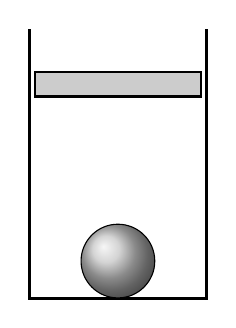
\begin{tikzpicture}[>=stealth,scale=0.9]
\draw[line width=1.2pt] (0,3.8)--(0,0)--(2.5,0)--(2.5,3.8);
\filldraw[fill=gray!40,line width=0.9pt] (0.08,2.85) rectangle (2.42,3.2);
\shade[ball color=gray!45] (1.25,0.53) circle (0.52);
\draw (1.25,0.53) circle (0.52);
\end{tikzpicture}
\end{center}
В цилиндрическом сосуде под поршнем находится газ. Поршень не закреплён и может перемещаться в сосуде без трения. На дне сосуда лежит стальной шарик (см. рисунок). Газ нагревают. Как изменятся в результате этого давление газа и действующая на шарик сила Архимеда? Атмосферное давление неизменно.

Для каждой величины определите соответствующий характер изменения:
\begin{enumerate}
\item увеличится
\item уменьшится
\item не изменится
\end{enumerate}
\TaskChangeTable{Давление газа}{Сила Архимеда}
}{
\smallskip\noindent\textbf{Решение от GPT}\par
Равновесие свободного поршня даёт \(p=p_{\text{атм}}+Mg/S\), где \(M\) — масса поршня, \(S\) — его площадь. Поэтому давление не изменится (\(3\)). При нагревании газ расширяется, его плотность \(\rho\) уменьшается. Следовательно, сила Архимеда \(F_A=\rho gV_{\text{ш}}\) уменьшится (\(2\)).

Ответ: \(32\).
}

% Source F68A6A: https://ege.fipi.ru/bank/questions.php?search=1&proj=BA1F39653304A5B041B656915DC36B38&qid=F68A6A
\BankTask{F68A6A}{
Необходимо собрать экспериментальную установку, с помощью которой можно определить плотность бензина. Для этого школьник взял стакан с бензином и динамометр.

Какие два предмета из приведённого ниже перечня оборудования необходимо дополнительно использовать для проведения этого эксперимента?
\begin{enumerate}
\item[1)] калориметр
\item[2)] мензурка
\item[3)] стальной цилиндр с крючком
\item[4)] термометр
\item[5)] пружина
\end{enumerate}
}{
\smallskip\noindent\textbf{Решение от GPT}\par
Нужны мензурка (2) и стальной цилиндр с крючком (3): объём цилиндра \(V\) определяют по объёму вытесненного бензина. Измерив динамометром вес цилиндра в воздухе \(P_1\) и при полном погружении в бензин \(P_2\), находят \(\rho=(P_1-P_2)/(gV)\). Калориметр (1) и термометр (4) не нужны, а пружина (5) не даёт необходимых измерений объёма погружённого тела. Ответ: 2, 3.
}

% Source A6D7D1: https://ege.fipi.ru/bank/questions.php?search=1&proj=BA1F39653304A5B041B656915DC36B38&qid=A6D7D1
\BankTask{A6D7D1}{
Ученик изучает силу Архимеда, действующую на тела, полностью погружённые в жидкость. В его распоряжении имеется пять установок, состоящих из ёмкости с жидкостью и сплошного шарика. Какие две из перечисленных в таблице установок необходимы ученику для того, чтобы на опыте обнаружить, зависит ли сила Архимеда от плотности материала шарика?
\begin{center}
\begin{tabular}{|c|c|c|c|}
\hline
\shortstack{№\\установки} & \shortstack{Жидкость, налитая\\в ёмкость} & Объём шарика & \shortstack{Материал, из которого\\сделан шарик} \\
\hline
1 & вода & $30\,\text{см}^{3}$ & сталь \\
\hline
2 & вода & $20\,\text{см}^{3}$ & алюминий \\
\hline
3 & керосин & $20\,\text{см}^{3}$ & алюминий \\
\hline
4 & подсолнечное масло & $30\,\text{см}^{3}$ & сталь \\
\hline
5 & вода & $30\,\text{см}^{3}$ & алюминий \\
\hline
\end{tabular}
\end{center}
}{
\smallskip\noindent\textbf{Решение от GPT}\par
Нужно взять шарики одинакового объёма из разных материалов и полностью погрузить их в одну и ту же жидкость. Этим требованиям соответствуют установки 1 и 5: вода, объём $30\,\text{см}^{3}$, материалы — сталь и алюминий. Сила Архимеда $F_A=\rho_{\text{ж}}gV$ в обоих опытах одинакова и не зависит от плотности материала шарика. Ответ: 1 и 5.
}

% Source 29874: https://phys-ege.sdamgia.ru/problem?id=29874
\BankTask{29874}{
Однородный деревянный шар массой $m=1{,}6$ кг лежит в сосуде с водой, касаясь дна и не касаясь стенок сосуда, так, что половина шара находится в воде. Определите плотность дерева, если шар  давит на дно с силой $F=6$ Н. Сделайте рисунок с указанием сил, действующих на шар.
}{
\smallskip\noindent\textbf{Решение}\par
\begin{center}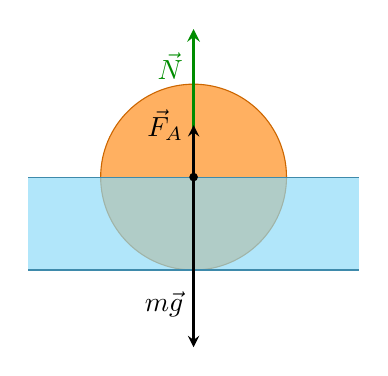
\begin{tikzpicture}[>=stealth]
\filldraw[fill=orange!62,draw=orange!80!black] (0,0) circle (1.18);
\fill[cyan!45,opacity=.68] (-2.1,-1.18) rectangle (2.1,0);
\draw[cyan!65!black] (-2.1,0)--(2.1,0) (-2.1,-1.18)--(2.1,-1.18);
\fill (0,0) circle (.055);
\draw[->,line width=1pt,green!55!black] (0,0)--(0,1.88) node[left,near end] {$\vec N$};
\draw[->,thick] (0,0)--(0,.66) node[left] {$\vec F_A$};
\draw[->,thick] (0,0)--(0,-2.16) node[left,near end] {$m\vec g$};
\end{tikzpicture}\end{center}
 Сила, с которой шар давит на дно, равна по модулю силе реакции опоры по третьему закону Ньютона $F=N.$ Изобразим силы, действующие на деревянный шар (см. рис). 
Шар находится в равновесии, следовательно, $N + F_A=m g.$ Сила Архимеда при погружении шара наполовину, $F_A=\rho_0 g \frac{V}{2} .$ Объем шара $V= \frac{m}{\rho} .$ Объединив формулы, находим плотность дерева, из которого изготовлен шар: 

\[\rho= \frac{\rho_0 g m}{2 \cdot ( m g - N )} = \frac{10 ^3 \cdot 10 \cdot 1{,}6}{2 \cdot ( 1{,}6 \cdot 10 - 6 )} =800 \frac{\,\text{кг}}{\,\text{м} ^3} .\]

Ответ: $800\,\text{кг/м}^{3}$.
}

% Source 41563: https://phys-ege.sdamgia.ru/problem?id=41563
\BankTask{41563}{
\begin{center}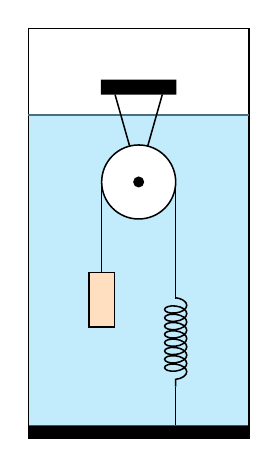
\begin{tikzpicture}[>=stealth,line width=.55pt]\fill[cyan!24](0,0)rectangle(2.8,4.1);\draw(0,0)rectangle(2.8,5.2);\draw[cyan!45!black](0,4.1)--(2.8,4.1);\fill(0,0)rectangle(2.8,.16) (.92,4.36)rectangle(1.88,4.55);\draw(1.1,4.36)--(1.4,3.3)--(1.7,4.36);\draw[fill=white](1.4,3.25)circle(.47);\fill(1.4,3.25)circle(.07);\draw(.93,3.25)--(.93,2.1) (1.87,3.25)--(1.87,1.77);\draw[fill=orange!25](.77,1.41)rectangle(1.09,2.1);\draw[decorate,decoration={coil,segment length=3pt,amplitude=4pt}](1.87,1.78)--(1.87,.65);\draw(1.87,.65)--(1.87,.16);\end{tikzpicture}\end{center}На рисунке представлена система тел, состоящая из неподвижного блока с перекинутой через него лёгкой и нерастяжимой нитью, к концам которой привязаны груз массой m  =  $0{,}8\,\text{кг}$ и объёмом V  =  $100\,\text{см}^{3}$ и лёгкая пружина жёсткостью k  =  $100$ H/м. Эта система находится в покое и  погружена в сосуд с жидкостью плотностью $\rho = 900\,\text{кг/м} ^3 .$ Нижний конец пружины прикреплён к дну сосуда. Как и на сколько изменится сила натяжения нити, действующая на пружину, если сосуд будет заполнен не первоначальной жидкостью, а таким же объёмом воды? Считать, что трение в оси блока отсутствует.
}{
\smallskip\noindent\textbf{Решение}\par
\begin{center}\begin{tikzpicture}[>=stealth,line width=.55pt]\fill[cyan!24](0,0)rectangle(2.8,4.1);\draw(0,0)rectangle(2.8,5.2);\draw[cyan!45!black](0,4.1)--(2.8,4.1);\fill(0,0)rectangle(2.8,.16) (.92,4.36)rectangle(1.88,4.55);\draw(1.1,4.36)--(1.4,3.3)--(1.7,4.36);\draw[fill=white](1.4,3.25)circle(.47);\fill(1.4,3.25)circle(.07);\draw(.93,3.25)--(.93,2.1) (1.87,3.25)--(1.87,1.77);\draw[fill=orange!25](.77,1.41)rectangle(1.09,2.1);\draw[decorate,decoration={coil,segment length=3pt,amplitude=4pt}](1.87,1.78)--(1.87,.65);\draw(1.87,.65)--(1.87,.16);\draw[->](-.25,5.18)--(-.25,.05)node[below]{$y$};\node[left]at(-.25,5.18){$0$};\draw[->](.93,1.77)--(.93,2.93)node[left]{$\vec T_1$};\draw[->](.93,1.77)--(.93,2.55)node[right]{$\vec F_{\text{арх}}$};\draw[->](.93,1.77)--(.93,.83)node[below]{$m\vec g$};\end{tikzpicture}\end{center}Изобразим силы, действующие на груз: сила тяжести $m\vec g,$ сила натяжения нити $\vec T_1,$ сила Архимеда $\vec F_A.$ По третьему закону Ньютона сила натяжения нити равна силе упругости, возникающей в пружине, равна силе натяжения $\vec T_1,$ так как нить легкая и сила трения в блоке отсутствует. В инерциальной системе отсчета, связанной с Землей, условие равновесия груза имеет вид:

\[m\vec g + \vec T_1 + \vec F_A=0.\]

В проекции на ось Oy: $T_1 + F_A - mg=0,$ где сила Архимеда равна $F_A=\rho gV.$ Откуда сила натяжения нити, действующая на груз, погруженный в жидкость, равна

\[T_1=mg - \rho gV.\]

Если  жидкость заменить на воду, то сила натяжения нити станет равной

\[T_2=mg - \rho_{\,\text{в}} gV.\]

Поскольку плотность воды  больше плотности жидкости, то сила Архимеда увеличится, а сила натяжения уменьшится на величину, равную

\[T_1 - T_2=gV ( \rho_{\,\text{в}} - \rho ) =10 \cdot 10 ^{ - 4 } \cdot ( 1000 - 900 ) =0{,}1\,\text{Н}.\]

Ответ: уменьшится на $0{,}1$ Н.
}

% Source 49644: https://phys-ege.sdamgia.ru/problem?id=49644
\BankTask{49644}{
Метеорологический зонд общей массой $20\,\text{кг}$ удерживают на поверхности Земли силой, равной по модулю $1$ кН и направленной вниз. Затем зонд отпускают, он поднимается вверх и остаётся на такой высоте, где его объём увеличивается в $2$ раза. Температура, измеренная зондом на этой высоте, равна –$43$ \ensuremath{{}^\circ}С. Определите давление на этой высоте, если на поверхности Земли давление равно $10^{5}$ Па, а температура равна +$17$ \ensuremath{{}^\circ}С.
}{
\smallskip\noindent\textbf{Решение}\par
На зонд, находящийся на Земле, действуют сила тяжести mg,  приложенная сила F, направленные вертикально вниз, сила Архимеда $F_{\,\text{арх}1,}$ направленная вертикально вверх. Зонд неподвижный, поэтому по второму закону Ньютона

\[F_{A1} = mg + F.\]

Сила Архимеда в этом случае равна $F_{A1}=\rho_1gV,$ где $\rho_1$ — плотность воздуха у поверхности Земли, V  — первоначальный объем зонда.
Плотность воздуха  найдем из уравнения Менделеева  — Клайперона $p_1 = \frac{\rho_1RT_1}{M} ,$ откуда $\rho_1 = \frac{p_1M}{RT_1} .$
Когда зонд поднимется на некоторую высоту, на него будут действовать сила тяжести и сила Архимеда $F_{\,\text{арх}}2 = \rho_2g \cdot 2V.$ Плотность воздуха на высоте находим аналогично из уравнения Менделеева  — Клапейрона $\rho_2 = \frac{p_2M}{RT_2} .$
Решая систему уравнений, находим давление на высоте:

\[p_2 = \frac{mgp_1T_2}{2T_1 ( mg + F )} = \frac{20 \cdot 10 \cdot 10 ^{5} \cdot 230}{2 \cdot 290 \cdot ( 20 \cdot 10 + 1000 )} \approx 6{,}6\,\text{кПа}.\]

Ответ: $6{,}6$ кПа.
}

% Source 43027: https://phys-ege.sdamgia.ru/problem?id=43027
\BankTask{43027}{
Общая масса газонепроницаемой оболочки воздушного шара и его корзины равна $400\,\text{кг}$. Шар заполнен гелием массой $100\,\text{кг}$. Он может поднять в воздух груз массой $225\,\text{кг}$. Какую минимальную массу гелия нужно добавить в оболочку шара, чтобы шар поднял еще одного пассажира массой $50\,\text{кг}$? Считать, что оболочка шара не оказывает сопротивления изменению его объема, воздушных течений в вертикальном направлении нет. Температура и давление гелия внутри шара и воздуха снаружи шара соответственно одинаковы.
}{
\smallskip\noindent\textbf{Решение}\par
Обозначим массу оболочки, гелия и груза $M=m_o + m_{\,\text{г}} + m.$ На шар действуют сила тяжести и выталкивающая сила со стороны воздуха. При поднятии шара подъемная сила равна 

\[F_{\,\text{под}}=F_A - Mg,\]

где выталкивающая сила $F_A=\rho_{\,\text{воз}}gV,$ V - объем шара. Плотность воздуха найдем из уравнения Менделеева-Клапейрона

$p= \frac{\rho_{\,\text{воз}}RT}{M_{\,\text{воз}}} ,$ откуда $\rho_{\,\text{воз}}= \frac{pM_{\,\text{воз}}}{RT} ,$

где p - давление наружного воздуха, T − температура воздуха снаружи шара.
Объем шара найдем из уравнения Менделеева-Клапейрона для гелия:

$pV= \frac{mRT}{M_{\,\text{г}}} ,$ откуда $V= \frac{mRT}{pM_{\,\text{г}}} ,$

где p - давление гелия, равное внешнему давлению, T - температура гелия, равная наружной температуре по условию.
Таким образом, подъемная сила шара равна:

\[F_{\,\text{под}}=g ( \frac{M_{\,\text{воз}}m}{M_{\,\text{г}}} - m_o - m - m_{\,\text{г}} ) =10 \cdot ( \frac{29 \cdot 10 ^{ - 3 } \cdot 100}{4 \cdot 10 ^{ - 3 }} - 400 - 100 - 225 ) =0.\]

Это означает, что масса поднимаемого груза является максимальной.
При добавлении пассажира и минимальной массы гелия в шар подъемная сила не изменится и будет выполняться аналогичное первому случаю соотношение:

\[m_o + m + m_{\,\text{г}} + m_{\,\text{п}}= \frac{M_{\,\text{воз}} ( m + \Delta m )}{M_{\,\text{г}}} .\]

При объединении соотношений для двух случаев получаем:

\[m_{\,\text{п}} + \Delta m= \frac{M_{\,\text{воз}}\Delta m}{M_{\,\text{г}}} ,\]

откуда находим минимальную массу гелия, который нужно добавить в шар:

\[\Delta m= \frac{m_{\,\text{п}}M_{\,\text{г}}}{M_{\,\text{воз}} - M_{\,\text{г}}} = \frac{50 \cdot 4 \cdot 10 ^{ - 3 }}{( 29 - 4 ) \cdot 10 ^{ - 3 }} =8\,\text{кг}.\]

Ответ: $8\,\text{кг}$.
}

% Source 9248: https://phys-ege.sdamgia.ru/problem?id=9248
\BankTask{9248}{
Мальчик решил подняться в воздух на воздушных шарах с гелием. Известно, что мальчик весит $40\,\text{кг}$, а на улице нормальное атмосферное давление и температура $27$ °C. Учитывая, что объем одного шара составляет $10$ литров, найдите, сколько потребуется шаров для такого путешествия. Массой оболочки шаров и объемом мальчика пренебречь.
}{
\smallskip\noindent\textbf{Решение}\par
На мальчика действуют силы: сила Архимеда $F_A=\rho_{\mathrm{He}} ( nV ) g,$ сила тяжести, действующая на человека, mg и сила тяжести, действующая на шарики, $m_{\mathrm{He}}g=\rho_{\mathrm{He}}g ( nV ) .$
Мальчик будет подниматься за счет силы Архимеда, действующей на шары:

$mg + m_{\mathrm{He}}g=F_A.$
$mg + \rho_{\mathrm{He}} ( nV ) g=g\rho_{\,\text{в}} ( nV ) ,$

откуда количество шариков:

\[n= \frac{m}{V ( \rho_{\,\text{в}} - \rho_{\mathrm{He}} )} ,\]

где $\rho_{\,\text{в}}$  — плотность воздуха, $\rho_{\mathrm{He}}$  — плотность гелия.
Из уравнения Менделеева  — Клапейрона можем найти плотность газа при данной температуре и давлении:

$p= \frac{\rho}{M} RT ,$
$\rho= \frac{pM}{RT} .$

Найдем необходимое количество шаров, учитывая, что гелий в шариках находится при той же температуре и давлении, что и воздух вокруг:

\[n= \frac{m}{V ( \rho_{\,\text{в}} - \rho_{\mathrm{He}} )} = \frac{mRT}{Vp_0 ( M_{\,\text{в}} - M_{\mathrm{He}} )} = \frac{40 \cdot 8{,}31 \cdot 300}{10 \cdot 10 ^{ - 3 } \cdot 10 ^{ 5 } \cdot ( 0{,}029 - 0{,}004 )} \approx 4000.\]

Ответ: $4000$.
}

% Source 7165: https://phys-ege.sdamgia.ru/problem?id=7165
\BankTask{7165}{
\begin{center}\begin{tikzpicture}[task graph,>=stealth]\draw(0,1.45)circle(1.45);\draw(-1.3,.82)--(-.48,-1.18)--(.48,-1.18)--(1.3,.82);\draw(-.58,-.91)rectangle(.58,-1.18);\foreach \x in {-.5,-.34,...,.46}{\draw(\x,-.91)--++(.06,-.27);}\draw(-.09,-.91)--(-.09,-.14)..controls(-.7,.15)and(-.4,.34)..(-.56,.57)..controls(-.71,.91)and(-.18,.97)..(-.23,1.2)..controls(-.3,1.43)and(.27,1.64)..(.3,1.28)..controls(.57,1.11)and(.38,.83)..(.51,.65)..controls(.74,.35)and(.32,.3)..(.09,-.12)--(.09,-.91);\node at(.74,.9){\(t\)};\node at(-1.31,-.26){\(t_0\)};\end{tikzpicture}\end{center}
Воздушный шар, оболочка которого имеет массу M  =  $145\,\text{кг}$ и объем V  =  $230\,\text{м}^{3}$, наполняется горячим воздухом при нормальном атмосферном давлении и температуре окружающего воздуха $t_{0}$  =  $0$ °С. Какую минимальную температуру t должен иметь воздух внутри оболочки, чтобы шар начал подниматься? Оболочка шара нерастяжима и имеет в нижней части небольшое отверстие.
}{
\smallskip\noindent\textbf{Решение}\par
На шар действуют: сила Архимеда $F_A=\rho_{\,\text{в}}gV,$ сила тяжести, действующая на воздух внутри, $mg$ и сила тяжести, действующая на оболочку, $Mg.$ По второму закону Ньютона:

\[\vec F_A + m \vec{g} + M \vec{g}=0.\]

В  проекциях на вертикаль: $F_A=mg + Mg.$
Условие подъема шара: $F_{\,\text{Арх}}. > \,\text{или} \,\text{равно} Mg + mg,$ где M  — масса оболочки, $m=\rho V$— масса воздуха внутри оболочки, отсюда:

$\rho_0gV > \,\text{или} \,\text{равно} Mg + \rho gV,$
$\rho_0V > \,\text{или} \,\text{равно} M + \rho V,$

где \ensuremath{\rho}$_{0}$  — плотность окружающего воздуха, \ensuremath{\rho} — плотность воздуха внутри оболочки, V  — объем шара.
Для воздуха внутри шара находим: $\frac{pV}{T} = \frac{m}{\mu} R,$ или $\frac{m}{V} = \frac{p \cdot \mu}{R \cdot T} = \rho,$ где p  — атмосферное давление, $\mu$  — молярная масса воздуха, T  — температура воздуха внутри шара. Соответственно, имеем плотность воздуха снаружи: $\rho_0= \frac{\mu p}{RT_0} ,$ где $T_{0}$  — температура окружающего воздуха.

$\frac{p \cdot \mu \cdot V}{R \cdot T_0} > \,\text{или} \,\text{равно} M + \frac{p \cdot \mu \cdot V}{R \cdot T} .$
$\frac{p \cdot \mu \cdot V}{R \cdot T_{\min}} = \frac{p \cdot \mu \cdot V}{R \cdot T_0} - M.$
$\frac{1}{T_{\min}} = \frac{1}{T_0} - \frac{M \cdot R}{p \cdot \mu \cdot V} ,$

$T_{\min}=T_0 \frac{p\mu V}{p\mu V - MRT_0} =273 \cdot \frac{10 ^{5} \cdot 29 \cdot 10 ^{ - 3 } \cdot 230}{10 ^{5} \cdot 29 \cdot 10 ^{ - 3 } \cdot 230 - 145 \cdot 8{,}31 \cdot 273} \approx 538\,\text{К} = 265 ^\circ \,\text{С}.$

Ответ: $265$.
}

% Source 29463: https://phys-ege.sdamgia.ru/problem?id=29463
\BankTask{29463}{
\begin{center}\begin{tikzpicture}[task graph,>=stealth]\fill[cyan!22](0,2.95)--(0,.54)arc(180:270:.54)--(3.85,0)arc(270:360:.54)--(4.39,2.95)--cycle;\draw(0,3.5)--(0,.54)arc(180:270:.54)--(3.85,0)arc(270:360:.54)--(4.39,3.5);\draw(0,2.95)--(4.39,2.95);\draw[fill=white](1.02,1.43)rectangle(3.08,2.73);\foreach \x in {1.13,1.34,...,2.86}{\foreach \y in {1.56,1.78,...,2.63}{\fill[gray](\x,\y)circle(.24pt);}}\draw(3.08,2.73)--(3.68,2.73)(3.08,1.43)--(3.68,1.43);\draw[fill=orange!30](3.14,1.43)rectangle(3.39,2.73);\draw(1.12,1.23)circle(.1)(3.16,1.23)circle(.1);\draw(1.12,1.43)--(1.12,1.33)(3.16,1.43)--(3.16,1.33)(1.18,1.15)--(2.16,.14)--(3.1,1.15)(2.16,.14)--(2.16,0);\foreach \x/\y in {.31/2.63,.32/1.78,.34/1.15,.53/.34,3.6/2.52,3.72/1.83,3.69/.98,2.8/.35}{\draw[cyan!55!black](\x,\y)--++(.34,0);}\end{tikzpicture}\end{center}
Сосуд с воздухом, отделенным от атмосферы поршнем, поместили в сосуд с водой и прикрепили ко дну кастрюли нитью, не дающей сосуду всплыть на поверхность. Начальная температура воздуха в сосуде и воды в кастрюле $t_{1}$  =  $18$ °C. Кастрюлю помещают в холодильник. Ниже какой температуры $t_{2}$ должна охладиться вода, чтобы сосуд опустился на дно кастрюли?
Начальный объем воздуха в сосуде $V_{1}$  =  $2$ дм$^{3}$. Масса сосуда с поршнем m  =  $2{,}2\,\text{кг}$. Сосуд и поршень изготовлены из стали, плотность которой $\rho = 7800 \,\text{кг/м} ^3 .$ Поршень может скользить без трения со стенками сосуда. Считать массу воздуха в сосуде намного меньшей, чем масса сосуда с поршнем.
}{
\smallskip\noindent\textbf{Решение}\par
$1$.  В сосуде с воздухом по условию поршень может скользить без трения. Значит, он будет перемещаться до тех пор, пока внешнее и внутреннее давление не станут равными. Учитывая, что глубина кастрюли небольшая, внешнее давление на поршень существенно не изменится. Поэтому процесс охлаждения воздуха в сосуде можно считать изобарным. Тогда по закону Гей-Люссака:

\[\frac{V_1}{V_2} = \frac{T_1}{T_2} ,\]
 откуда:

\[T_2= \frac{V_2}{T_1} V_1.\]

$2$.  При начальной температуре воды на сосуд действуют сила Архимеда, направленная вверх, сила тяжести сосуда, направленная вниз, и результирующая сил натяжения нитей, направленная вниз. С учетом того, что масса воздуха намного меньше массы сосуда с поршнем, силой тяжести, действующей на воздух можно пренебречь. 
$3$.  При понижении температуры воды, воздух в сосуде будет изобарно охлаждаться, объем воздуха уменьшится. Тогда уменьшится суммарный объем воздуха и сосуда. Силы натяжения нитей станут равными нулю. Тело будет тонуть при условии, что $F_A < mg.$ Сила Архимеда, действующая на тело, равна $F_A=\rho _0gV,$ где $V=V_c + V_2.$ Объем сосуда с поршнем $V_c= \frac{m}{\rho} .$ 
$4$.  Объединяя уравнения и неравенство, получаем:

\[\rho _0 ( \frac{m}{\rho} + V_2 ) < m,\]
 откуда:

\[V_2 < \frac{m ( \rho - \rho _0 )}{\rho\rho _0} .\]

Следовательно, температура воды должна быть:

$T_2 < \frac{m ( \rho - \rho _0 ) T_1}{\rho \rho _0V_1} = \frac{2{,}2\,\text{кг} \cdot ( 7{,}8 - 1 ) \cdot 10 ^3 \,\text{кг/м} ^3 \cdot 291\,\text{К}}{10 ^3 \,\text{кг/м} ^3 \cdot 7{,}8 \cdot 10 ^3 \,\text{кг/м} ^3 \cdot 2 \cdot 10 ^{ - 3 } \,\text{м} ^3} \approx 279\,\text{К}$ или $t_2 < 6 ^\circ C.$

Ответ: ниже $6 ^\circ C.$
}

% Source 51478: https://phys-ege.sdamgia.ru/problem?id=51478
\BankTask{51478}{
К концам невесомого рычага подвесили за невесомые нерастяжимые нити два сплошных груза массами $1{,}28\,\text{кг}$ и $0{,}32\,\text{кг}$ и привели рычаг в состояние равновесия. Затем рычаг с грузами расположили над водой так, что оба груза целиком оказались под водой. В результате для сохранения равновесия точку опоры пришлось переместить на $10\,\text{см}$. Определите первоначальное расстояние от более тяжёлого груза до точки опоры, если объёмы обоих грузов одинаковы и равны $200\,\text{см}^{3}$. Сделайте рисунок, на котором укажите силы, действующие на рычаг (для двух случаев), а также на погружённые в воду грузы.
Обоснуйте применимость законов, используемых для решения задачи.
}{
\smallskip\noindent\textbf{Решение}\par
Обоснование.
$1$.  Рассмотрим задачу в системе отсчёта, связанной с Землёй. Будем считать эту систему отсчёта инерциальной  — ИСО.
$2$.  Опишем рычаг моделью абсолютно твёрдого тела  — форма и размеры тела неизменны, расстояние между любыми двумя точками тела остаётся неизменным.
$3$.  Сумма приложенных к абсолютно твёрдому телу внешних сил равна нулю, так как тело не совершает поступательного движения.
$4$.  Сумма моментов внешних сил относительно осей, проходящих через точки O$_{1}$ и O$_{2}$ перпендикулярно плоскости рисунка, равна нулю, так как тело не совершает вращательного движения.
$5$.  Грузы на нитях могут двигаться поступательно, поэтому опишем грузы моделью материальной точки и используем второй закон Ньютона.
$6$.  Нити невесомы, поэтому натяжение нити всюду одинаково.
$7$.  Согласно третьему закону Ньютона силы, с которыми взаимодействуют грузы, нити и рычаг, равны по модулю и направлены в противоположные стороны.
\begin{center}\begin{tikzpicture}[task graph,>=stealth]\draw[fill=gray!10](0,0)rectangle(6,.17);\draw(2,.17)--(1.73,.63)--(2.27,.63)--cycle;\foreach \x in {1.52,1.68,...,2.48}{\draw(\x,.63)--++(.14,.14);}\node[below right]at(2,0){\(O_1\)};\draw[->] (2,.63)--(2,1.54) node[above]{\(\vec Q_1\)};\draw[<->](0,-.54)--(2,-.54)node[midway,above]{\(l_1\)};\draw[<->](2,-.54)--(6,-.54)node[midway,above]{\(l_2\)};\draw(0,0)--(0,-1.39);\draw[fill=gray!15](0,-1.9)circle(.51);\draw[->] (0,0)--(0,-1.18) node[left]{\(\vec P_1\)};\draw(6,0)--(6,-1.39);\draw[fill=gray!30](6,-1.9)circle(.51);\draw[->] (6,0)--(6,-1.18) node[right]{\(\vec P_2\)};\draw[dashed](2,.3)--(2,-4.6);\draw[<->](1.2,-2.27)--(2,-2.27)node[midway,above]{\(\Delta l\)};\begin{scope}[yshift=-4cm]\draw[fill=gray!10](0,0)rectangle(6,.17);\draw(1.2,.17)--(0.93,.63)--(1.47,.63)--cycle;\foreach \x in {0.72,0.88,...,1.68}{\draw(\x,.63)--++(.14,.14);}\node[below right]at(1.2,0){\(O_2\)};\draw[->] (1.2,.63)--(1.2,1.54) node[above left]{\(\vec Q_2\)};\draw[<->](0,-.54)--(1.2,-.54)node[midway,above]{\(l_1-\Delta l\)};\draw[<->](1.2,-.54)--(6,-.54)node[midway,above]{\(l_2+\Delta l\)};\fill[blue!16](-.8,-3.3)rectangle(6.8,-1.27);\draw(-.8,-1.27)--(6.8,-1.27);\draw(0,0)--(0,-1.39);\draw[fill=gray!15](0,-1.9)circle(.51);\draw[->] (0,0)--(0,-1.18) node[left]{\(\vec P_1'\)};\draw[->] (0,-1.39)--(0,-1.12) node[above right]{\(\vec N_1'\)};\draw[->] (0,-1.9)--(0,-1.55) node[below right]{\(\vec F_{\text{Арх}}\)};\draw[->] (0,-1.9)--(0,-3.17) node[below left]{\(m_1\vec g\)};\draw(6,0)--(6,-1.39);\draw[fill=gray!30](6,-1.9)circle(.51);\draw[->] (6,0)--(6,-1.18) node[right]{\(\vec P_2'\)};\draw[->] (6,-1.39)--(6,-1.12) node[above left]{\(\vec N_2'\)};\draw[->] (6,-1.9)--(6,-1.55) node[below left]{\(\vec F_{\text{Арх}}\)};\draw[->] (6,-1.9)--(6,-3.17) node[below right]{\(m_2\vec g\)};\end{scope}\end{tikzpicture}\end{center}
Решение.
$1$.  Начальное условие равновесия $P_1 l_1 = P_2 l_2 ( 1 ) ,$ где $\overrightarrow{P}_i$  — силы, с которыми нити действуют на рычаг, l$_{i}$  — плечи рычага.
На каждый груз действуют только сила тяжести $m \vec g$ и сила реакции подвеса $\overrightarrow{N}.$ Нити невесомы, поэтому по третьему закону Ньютона $P = T,$ $T = N.$ Следовательно, $P = mg.$
$2$.  Когда грузы находятся в воде, на них действует архимедова сила $\overrightarrow{F}_{\,\text{Арх}},$ и в равновесии $N' = mg - F_{\,\text{Арх}},$ откуда

\[P' = mg - F_{\,\text{Арх}} = P - F_{\,\text{Арх}}.\]

$3$.  Под действием сил $\overrightarrow{P}_1$ и $\overrightarrow{P}_2$ рычаг находился в равновесии. В результате погружения грузов в воду обе силы уменьшились на одну и ту же величину. Следовательно, большая сила изменилась на меньшую относительную величину. Таким образом, для сохранения равновесия рычага в новых условиях надо уменьшить плечо большей силы.
Условие равновесия рычага в конечном состоянии: $P'_1 ( l_1 - \Delta l ) = P'_2 ( l_2 + \Delta l ) ,$ или

\[( P_1 - F_{\,\text{Арх}} ) ( l_1 - \Delta l ) = ( P_2 - F_{\,\text{Арх}} ) ( l_2 + \Delta l ) , \qquad ( 2 )\]

где F$_{\,\text{Арх}}$  — архимедова сила, $F_{\,\text{Арх}} = \rho gV.$
$4$.  Из уравнений $1$ и $2$ находим выражение для плеча l$_{1}$:

\[l_1 = \frac{\Delta l ( P_2 + P_1 - 2F_{\,\text{Арх}} )}{F_{\,\text{Арх}} ( \frac{P_1}{P_2} - 1 )} = \frac{\Delta l ( m_1 + m_2 - 2 \rho V )}{\rho V ( \frac{m_1}{m_2} - 1 )} = \frac{0{,}1 ( 1{,}28 + 0{,}32 - 2 \cdot 10 ^3 \cdot 2 \cdot 10 ^{ - 4 } )}{10 ^3 \cdot 2 \cdot 10 ^{-4} ( \frac{1{,}28}{0{,}32} - 1 )} = 0{,}2 \,\text{м}.\]

Ответ: $l_1 = 0{,}2 \,\text{м}.$
}

\end{document}
